\section{Design}

\subsection{Barrel layout and support structure}

SVT comprises 21504 channels of silicon strip sensors in six layers (three concentric polygonal regions that have 10, 14, and 18 double sided modules). 
To minimize multiple scattering a unique module design with extra long 33~cm strips has been developed to reduce material budget to about 1.4$\%$ of radiation length per region (two silicon planes) for normal incidence tracks, which is essential for tracking at low momenta. 

\begin{wrapfigure}{l}{0.5\columnwidth}
\centering 
\includegraphics[width=0.5\columnwidth]{barrel-faradaycage.png}
\caption{Layout of the barrel and the Faraday Cage. Copper supports shown in yellow.  Supports are bolted directly to cold plate. Silicon sensors are shown in green.}
\label{fig:barrel-faradaycage}
\end{wrapfigure}

All SVT modules are made identical to minimize the production cost. There are no overlaps of adjacent modules. The SVT modules are cantilevered off a water-chilled cold plate, designed to remove the heat generated by the electronics, located only at one end of the module outside of the tracking volume. The cold plate is bolted to the mounting tube which is attached to the insertion cart with the support tube. Alignment rods are used for adjustment. The cart hosts all detector services and is movable along the beam axis for easy maintenance.

%\begin{wrapfigure}{l}{0.5\columnwidth}
%\centering 
%\includegraphics[width=0.5\columnwidth]{cvt-crosssection.png}
%\caption{CVT crossection.}
%\label{fig:cvt-crosssection}
%\end{wrapfigure}

%Figure~\ref{fig:cvt-crosssection} shows the side view of the detector. 

The modules  are mounted between the upstream and the downstream rings (Figure~\ref{fig:barrel-faradaycage}). For each region the upstream ring is attached to the cold plate. The cold plate and upstream ring are mounted to a mounting tube. The mounting surfaces of the upstream and downstream rings are machined in a single step to guarantee planarity. The rings of each region are independent from each other to prevent overconstraining the assembly.  Regions are shifted along the beam axis to ensure angular coverage. This design allows an entire region to be removed as a unit, rather than module by module. Downstream rings are made of PolyEther Ether Ketone (PEEK)~\cite{NIMVCC}. 

\begin{figure}[hbt] 
\centering 
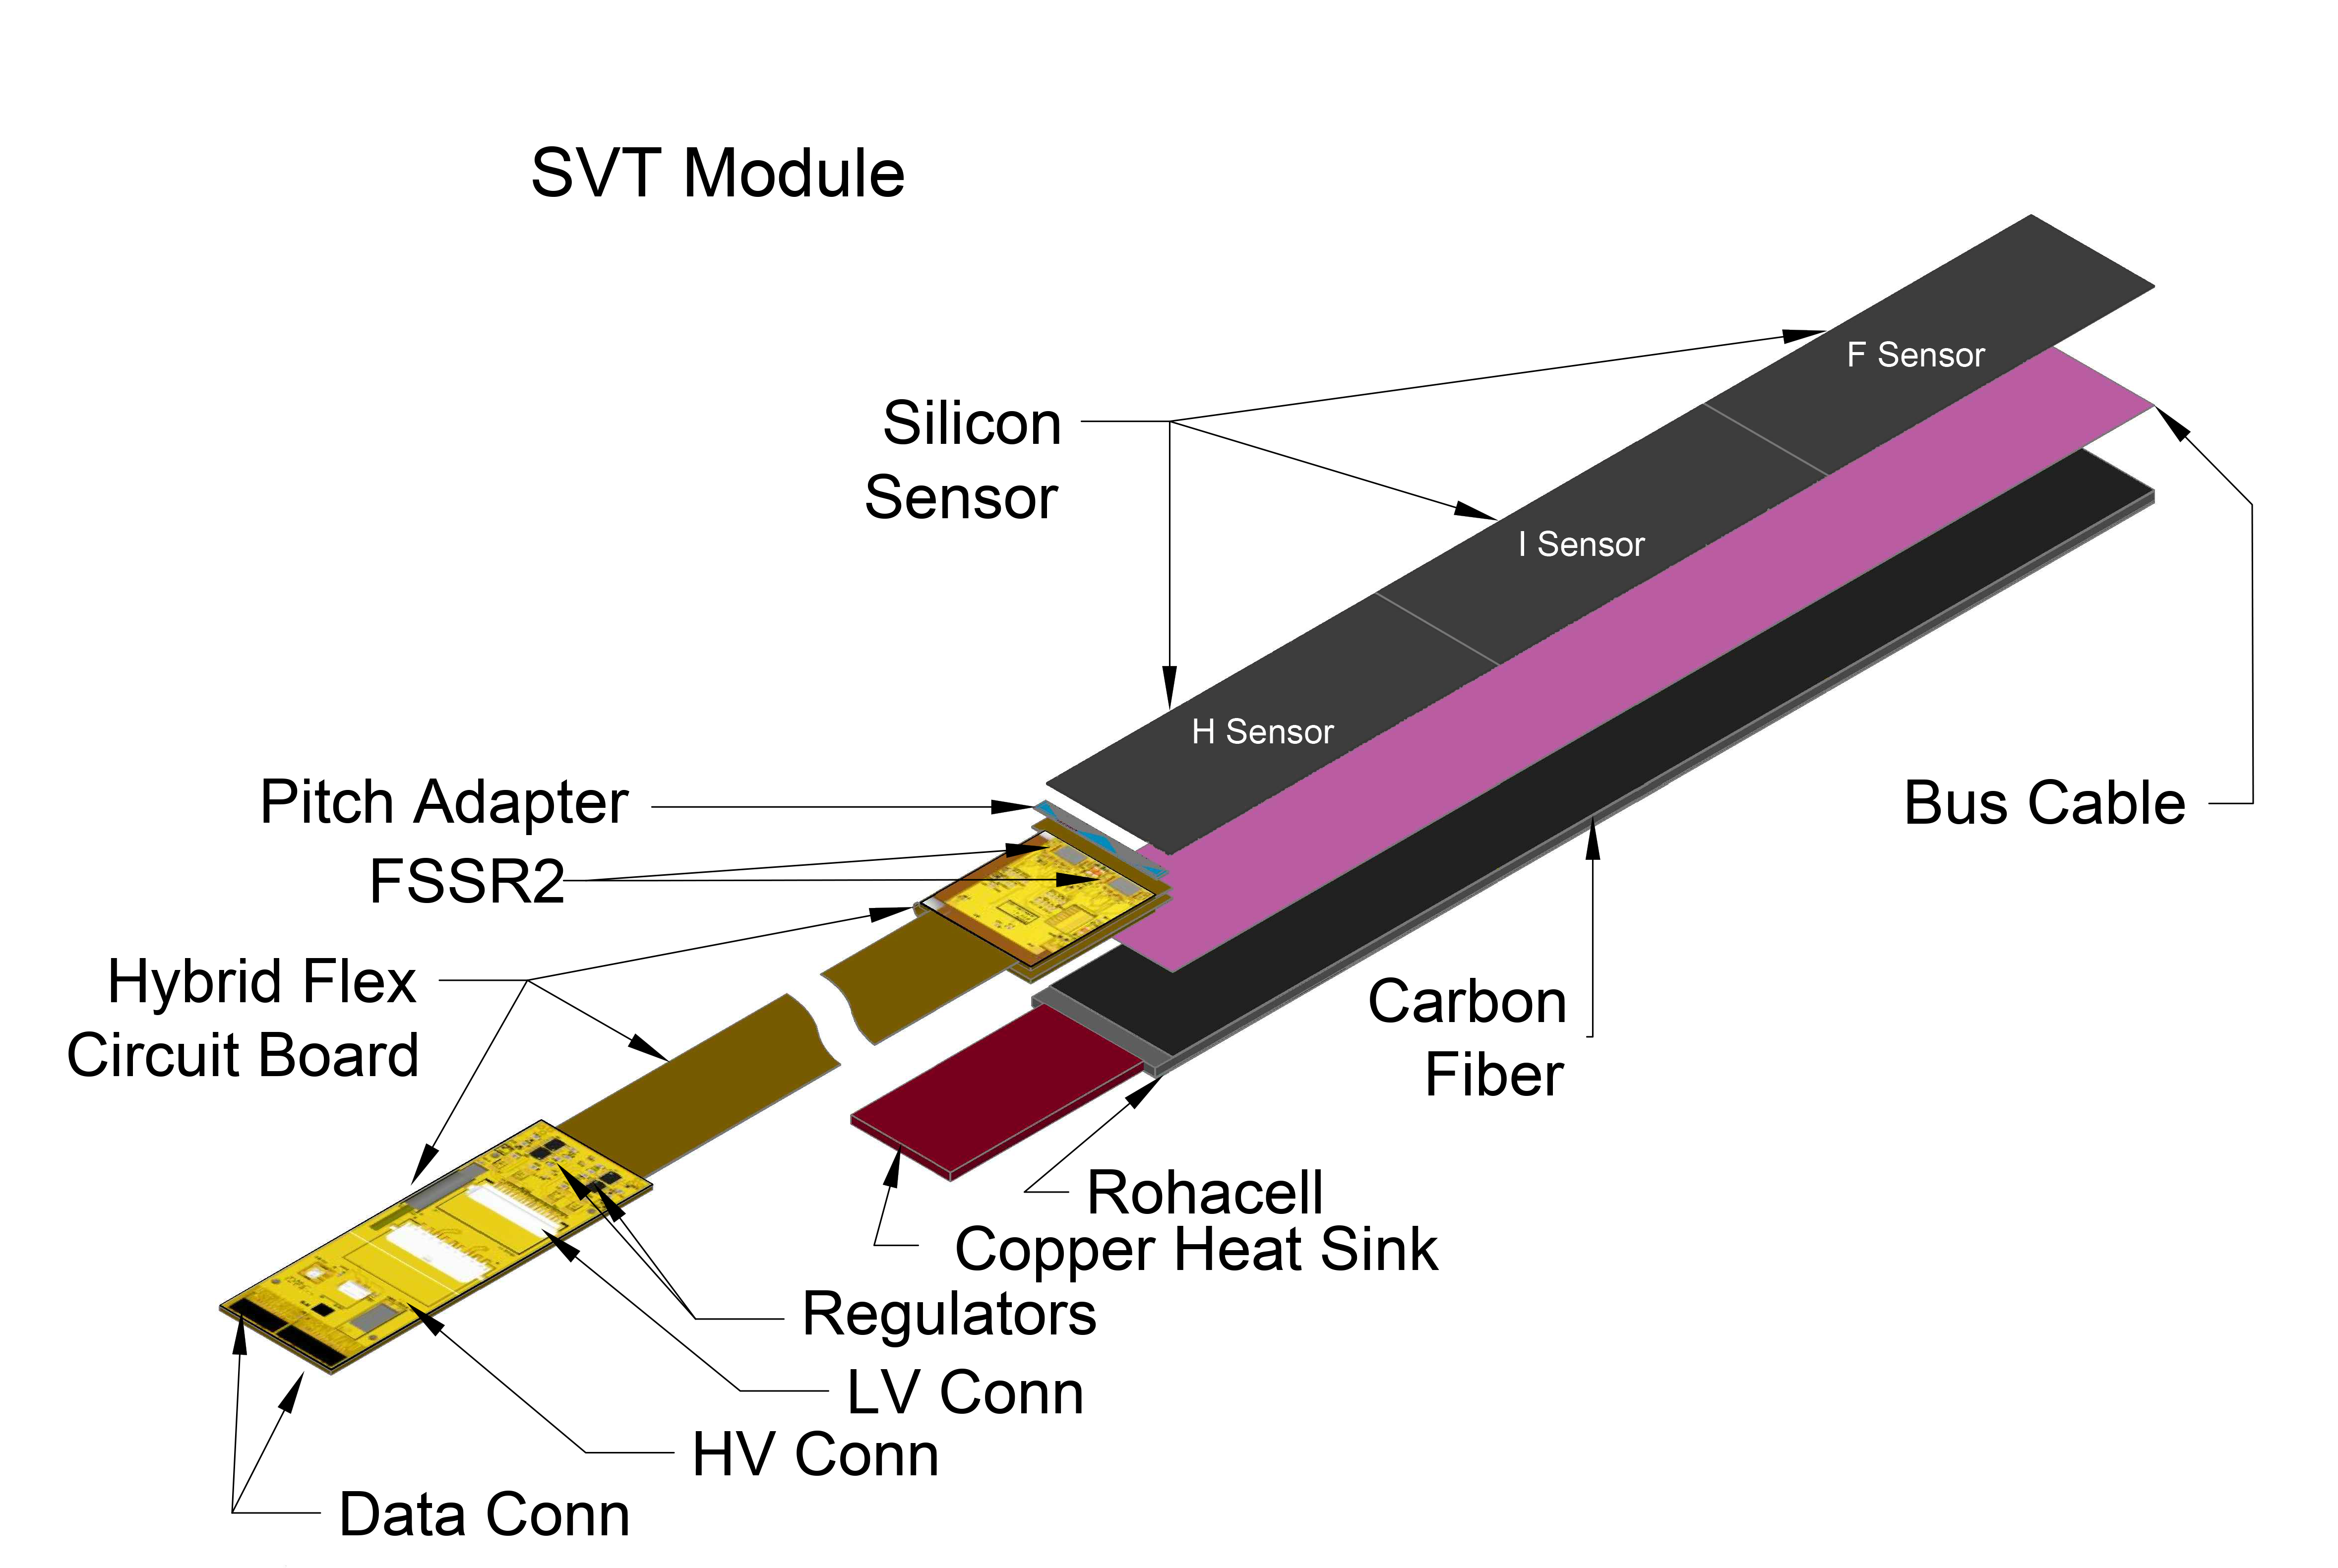
\includegraphics[width=1.0\columnwidth,keepaspectratio]{module.pdf}
\caption{Layout of the SVT module.}
\label{fig:module}
\end{figure}

\subsection{Module design}

SVT uses single sided 320~$\mu$m thick microstrip sensors fabricated by Hamamatsu mounted on each side of the module (see Fig.~\ref{fig:module}). All modules have 3 types of sensors: Hybrid, Intermediate, and Far. Sensors are cut from 6 inch wafers, 2 sensors per wafer to maximize the yield. All sensors have the same size, 112$\times$42 mm. There are three daisy-chained sensors per layer (six per module) with 110~$\mu$m gap between them. 

\begin{figure}[hbt] 
\centering 
\includegraphics[width=1.0\columnwidth,keepaspectratio]{strip-layout.png}
\caption{Sensor strip layout.}
\label{fig:strip-layout}
\end{figure}

Each layer has 256 strips with linearly varying angles of 0$^\circ$--3$^\circ$ (constant $\phi$ pitch of 1/85$^\circ$) to minimize dead sensor area. First readout strip is parallel to the longitudinal axis of the module; the last readout strip has an angle of 3$^\circ$ with respect to this axis (see Fig.~\ref{fig:strip-layout}). Because of the constant $\phi$ pitch, the lengths of the readout strips of the modules vary from 0.5 cm to 33 cm. At the hybrid side the intermediate strip pitch is 78 $\mu$m and the readout pitch is 156 $\mu$m The strip-to-pitch ratio is 0.256 for all three types of sensors.

\begin{wrapfigure}{l}{0.5\columnwidth}
\includegraphics[width=0.5\columnwidth]{backing-structure.png}
\caption{Backing structure.}
\label{fig:backing-structure}
\end{wrapfigure}

Sensors are mounted on a backing structure composed of Rohacell 71 core, bus cable, and carbon fiber (see Fig.~\ref{fig:backing-structure}). The carbon fiber skin is made from Mitsubishi type K13C2U fibers oriented in a quasi-isotropic (45/-45/0) pattern. To ensure adequate electrical conductivity it is co-cured with the bus cable, made from a Kapton sheet with 3 $\mu$m thick and 0.5~mm wide copper traces; one side provides high voltage to the sensors, a 6$\times$6~mm copper mesh on another side grounds the carbon fiber. 
The Rohacell core under the hybrid board is replaced by a copper heat sink to remove $\sim$2~W of heat generated by the ASICs. At the downstream end of the module, the Rohacell core is replaced by a PEEK insert.  

\begin{wrapfigure}{l}{0.5\columnwidth}
\includegraphics[width=0.5\columnwidth]{pitch-adapter.png}
\caption{One end of the pitch adapter mask, showing alignment fiducials, wire bonding pads, and traces.}
\label{fig:pitch-adapter}
\end{wrapfigure}

Pitch adapter matches the 156~$\mu$m sensor readout pitch to the 50~$\mu$m FSSR2 bonding pad pitch. The pitch adapter is a glass plate with metal traces made of an alloy of aluminum and copper. The alloy improves electromigration hardness and bonding. The metal layer is sputter deposited. The passivation silicon oxide layer protects the soft aluminum traces from damage. There are two fi ducials on the pitch adapter edge next to the sensor
and three on the edge next to the HFCB to facilitate alignment. The pitch adapter is 41.5 mm by 4 mm, with a tolerance of 50~$\mu$m. No more than one open trace or two short-circuited traces are allowed per pitch adapter. A section of the pitch adapter is shown in Figure~\ref{fig:pitch-adapter}. 
A readout system which instruments both sides of a module with a single rigid-flex Hybrid Flex Circuit Board (HFCB), has been developed by Jefferson Lab (see Fig.~\ref{fig:HFCB}) and fabricated by Compunetics Inc. The HFCB is located on the upstream end of the module. It hosts four FSSR2 ASICs, two on the top and two on the bottom side. The hybrid areas are connected by a 10~mm-long wing cable. The sensors, the pitch adapters, and the HFCB are glued with Huntsman TDR 1100-11 resin/hardener to both sides of the backing structure. The HFCB is wrapped around the backing structure with a wing cable (Fig.~\ref{fig:hfcb-wrap}). 

Data are transferred from the hybrid via the flex cable to the level one connect (L1C) board. The L1C has two high density Nanonics connectors for data and control lines, Molex Micro-Fit 9-pin connector for high voltage ($\sim$85~V) bias to the sensors, and AMP Mini CT 17 pin connector for low voltage (2.5~V) power to the ASICs. There are 12 layers in rigid part and 6 layers in flex part. Control, data, and clock signals do not cross the ground plane splits. Clock signals are located on a separate layer. Guard traces are routed between output, clock, and power lines. 

\begin{wrapfigure}{l}{0.5\columnwidth}
\includegraphics[width=0.5\columnwidth]{hfcb-wrap.png}
\caption{HFCB wrap}
\label{fig:hfcb-wrap}
\end{wrapfigure}

Separate planes are provided for analog and digital power. To reduce noise on these planes, regulators and bypass capacitors are added. High voltage filter circuits and the bridging of high and low voltage return lines are located close to the ASICs. Decoupling capacitors for power transmission are placed at transitions between flex and rigid materials. The HFCBs are routed through 10~mm radial slots in the cold plate. There are temperature and humidity sensors on each side of the HFCB for monitoring purposes.

\begin{figure}[hbt] 
\includegraphics[width=1.0\columnwidth]{HFCB.png}
\caption{Hybrid Flex Circuit Board (HFCB).}
\label{fig:HFCB}
\end{figure}

\subsection{Deflection}

The maximum deflection of a module due to gravity is 14~$\mu$m (Figure~\ref{fig:module-deflection}). The deflection of the downstream ring is less than 7~$\mu$m. The deflection of the entire SVT is 230~$\mu$m.

\begin{figure}[hbt] 
\includegraphics[width=0.8\columnwidth]{module-deflection.png}
\caption{Deflection of an individual module due to gravity.}
\label{fig:module-deflection}
\end{figure}

\subsection{Thermal analysis and heat removal}

For the thermal analysis, the module was modeled with the copper support and the heat sink insert. The heat output from each module is ~2 W. Cooling the cold plate with water, which flows around the fins of the heat sink inserts inside the cold plate at -20$^\circ$C, at a rate of 2 LPM, results in a temperature differential of the water between the inlet and outlet of the cold plate to be less than 1$^\circ$C. The temperature distribution on the module is shown in Figure~\ref{fig:module-temp}. The maximum temperature of the sensors at the readout end is -10$^\circ$C. The variation in temperature from the upstream end of the Hybrid sensor to the downstream end of the Far sensor is ~1$^\circ$C.

\begin{figure}[hbt] 
\centering 
\includegraphics[width=0.8\columnwidth,keepaspectratio]{module-temp.png}
\caption{Temperature distribution along the SVT module.}
\label{fig:module-temp}
\end{figure}
%\begin{wrapfigure}{l}{0.5\columnwidth}
%\includegraphics[width=0.5\columnwidth]{module-temp.png}
%\caption{Temperature distribution along the SVT module.}
%\label{fig:module-temp}
%\end{wrapfigure}

\subsection{Module Assembly and QA}
SVT modules are assembled at the Fermilab Silicon Detector Facility and tested at the Jefferson Lab. Prior to installation on a module, all components are inspected and tested as part of the quality assurance procedure.  
The layout of six bus cables on a panel has a minimum of 5.05 mm between adjacent cables on the panel to allow for the 1/8-inch diameter routing bit (Figure~\ref{fig:bus-cable-routing}).

%\begin{figure}[hbt] 
%\centering 
%\includegraphics[width=1.0\columnwidth,keepaspectratio]{bus-cable-routing.png}
%\caption{Cutting of the bus cable.}
%\label{fig:bus-cable-routing}
%\end{figure}
\begin{wrapfigure}{l}{0.4\columnwidth}
\includegraphics[width=0.4\columnwidth]{bus-cable-routing.png}
\caption{Cutting of the bus cable.}
\label{fig:bus-cable-routing}
\end{wrapfigure}

To assemble the backing structure, a mold and 3M Scotch-Weld 2216 epoxy that cures at room temperature is used.
The module has two pairs of mounting and fiducial holes in the copper heat sink and one in the PEEK insert. After module is fabricated, position of these fiducial holes is measured with respect to the fiducial marks etched on the sensor. Sensors are aligned with respect to insert fiducials within few micrometers. The holes for the mounting pin have a tight diameter tolerance and are used for module alignment. The slot in the PEEK insert has a tolerance of 5~$\mu$m. To accurately control the width of the backing structure, post-machining of the width at the downstream end and near the pitch adapter is done. After post-machining of the precision edge, any foam exposed due to that process is encapsulated with 3M DP190 epoxy. Edges of the backing structure are covered with Kapton tape to insulate the carbon fiber from the back side of the sensors. After installation of the HFCBs and pitch adapters, the module is placed in a box designed to allow storage of partially and fully fabricated modules.

\subsection{Detector integration and commissioning}

\begin{figure}[hbt]
\centering 
\includegraphics[width=1.0\columnwidth]{modulesupport.png}
\caption{SVT barrel assembly.}
\label{fig:modulesupport}
\end{figure}

Barrel integration took place at the Jefferson Lab. Regions are assembled in sequence. The assembly was done in a vertical position on a granite table. Modules are mounted on the dowels inserted in the rings by holding the module by the two handling rods which are screwed into the inserts (Fig.~\ref{fig:svt-assembly}). There are three fiducial points on each module, two on the upstream copper insert, and one on the downstream PEEK insert. During barrel assembly a survey of fiducial locations have been performed with precision of $\sim$20~$\mu$m using a FaroArm Quantum CMM. The shifts of survey positions from ideal geometry were taken into account by the alignment software. 
%(see Fig.~\ref{fig:survey}).

\begin{wrapfigure}{l}{0.5\columnwidth}
\includegraphics[width=0.5\columnwidth]{integration-cart.png}
\caption{Integration cart.}
\label{fig:integration-cart}
\end{wrapfigure}

\begin{wrapfigure}{l}{0.5\columnwidth}
\includegraphics[width=0.5\columnwidth]{svt-assembly.png}
\caption{SVT assembly}
\label{fig:svt-assembly}
\end{wrapfigure}

\begin{wrapfigure}{l}{0.5\columnwidth}
\includegraphics[width=0.5\columnwidth]{svt-assembled.png}
\caption{SVT after integration.}
\label{fig:svt-assembled}
\end{wrapfigure}

After assembling each region functionality of integrated modules was checked. When barrel assembly is complete, it was rotated to a horizontal position using a special fixture. (see Fig.~\ref{fig:rotation}).

\begin{wrapfigure}{l}{0.5\columnwidth}
\includegraphics[width=0.5\columnwidth]{barrel-assembled.png}
\caption{Assembled barrel}
\label{fig:barrel-assembled}
\end{wrapfigure}

%\begin{wrapfigure}{l}{0.5\columnwidth}
%\includegraphics[width=0.5\columnwidth]{survey.png}
%\caption{Survey}
%\label{fig:survey}
%\end{wrapfigure}
%
\begin{wrapfigure}{l}{0.5\columnwidth}
\includegraphics[width=0.5\columnwidth]{rotation.png}
\caption{Barrel rotation.}
\label{fig:rotation}
\end{wrapfigure}

The mounting tubes of the barrel are attached to the detector transportation cart, cable bundles routed along the support tubes and connected to the crates (see Fig.~\ref{fig:svt-assembled}).  

